\subsection{Vector Timing Correlation}
\label{sec:VTC}
\begin{figure}[t]
	\centering
	\vspace{-15pt}
	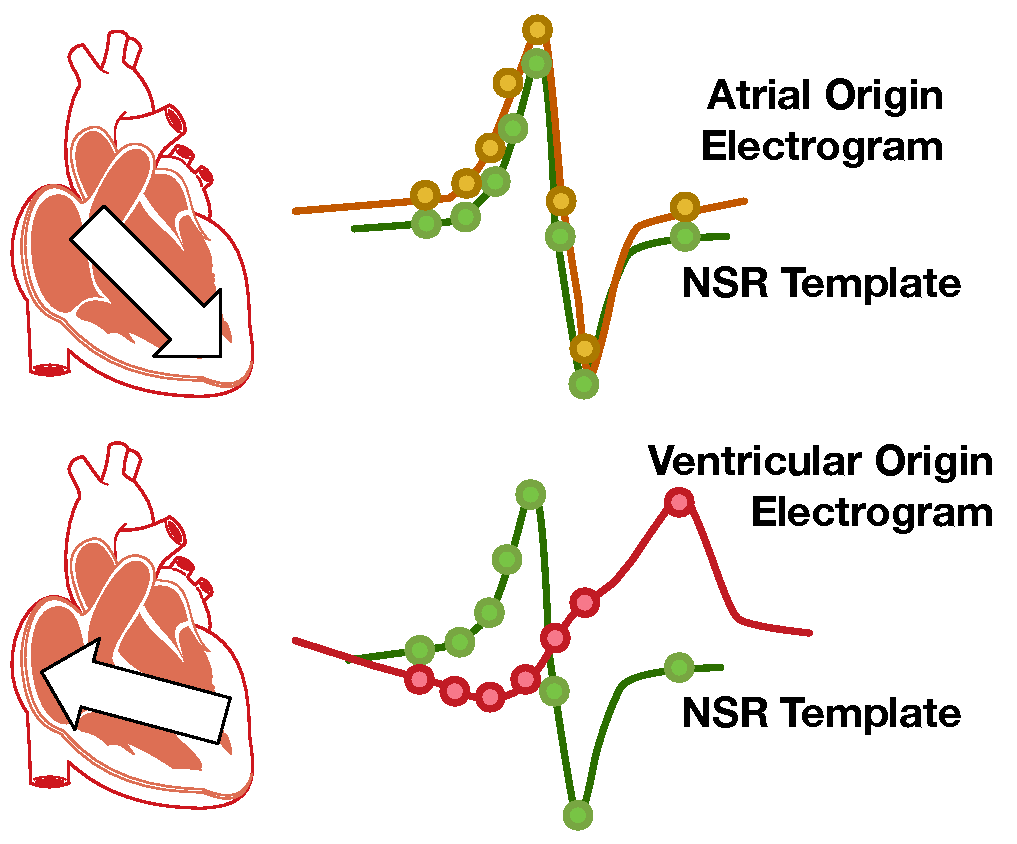
\includegraphics[scale=0.3]{figures/VTCEGMCompare}
	\caption{\small \acp{EGM} of different origin have different morphologies.}
	\label{fig:egmmorphology}
	\vspace{-10pt}
\end{figure}
%\caption{\small \acp{EGM} of different origin have different morphologies, while \acp{EGM} of same origin have very similar morphologies.}
It has been clinically observed that a depolarization wave originating in the ventricles (as produced during \ac{VT} for example) will in general produce a different \ac{EGM} morphology than a wave originating in the atria (as produced during \ac{SVT}) \cite{compass}.
See Fig. \ref{fig:egmmorphology}.
%
A morphology discriminator measures the correlation between the morphology of the current \ac{EGM} and that of a stored \emph{template} \ac{EGM} acquired during normal sinus rhythm.
If the correlation is above a pre-set threshold for a minimum number of beats, then this is an indication that the current arrhythmia is supraventricular in origin.
Otherwise, it might be of ventricular origin.

Boston Scientific's implementation of a morphology discriminator is called Vector and Timing Correlation (VTC).
VTC first samples 8 \emph{fiducial} points $\egm_i,i=1,\ldots,8$ on the current \ac{EGM} $\egm$ at pre-defined time instants.
Let $\egm_{m,i}$ be the corresponding points on the template \ac{EGM}.
A simple 0-shift correlation $\rho_{new}$ is calculated between the two sequences. 
If 3 out of the last 10 calculated correlation values exceed the threshold, then \ac{SVT} is decided and therapy is withheld.

The system of Fig. \ref{fig:HVTC} implements the VTC discriminator.
As before, $t$ is a local clock.
$\mu$ accumulates the values of the current \ac{EGM}, $\alpha$ accumulates the product $\egm_i \egm_{m,i}$, 
$\beta$ accumulates $\egm_i^2$.
State $w$ is an auxiliary state we need to establish the STORMED property.
$\vec{\nu}$ is a 10D binary vector: $\nu_i = -1$ if the $i^{th}$ correlation value fell below the threshold, and is $+1$ otherwise.
$L_3$ is the state of $\Sys_{TCFI}$: the guard condition $L_3 \leq th$ indicates that all its entries have values less than the tachycardia threshold, which is when $\Sys_{VTC}$ starts computing.
$WindowEnds$ indicates the `end' of an \ac{EGM}, measured as a window around the peak sensed by $\Sys_{Sense}$.  
%
\begin{figure}[t]
\centering
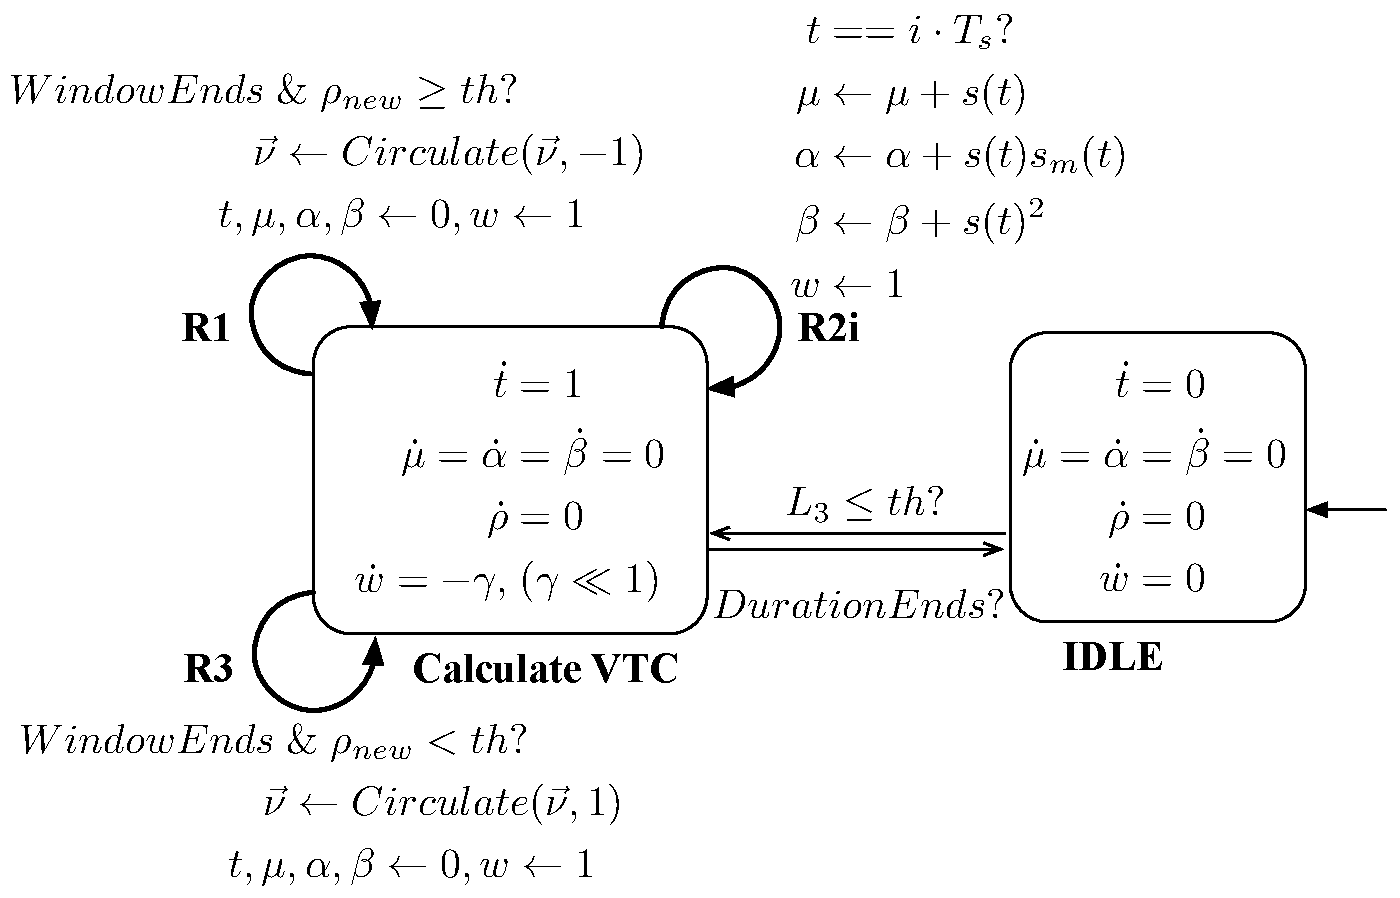
\includegraphics[scale=0.325]{figures/VTC1v2}
\vspace{-10pt}
\caption{VTC calculation. $iT_s$ is the sampling time for the $i${th} fiducial point, $i=1,\ldots,8$. $R2_{1},\ldots,R2_{8}$ are the corresponding resets. For clarity of the figure, 8 transitions are represented on the same edge.}
\vspace{-10pt}
\label{fig:HVTC}
\end{figure}
%
\begin{lemma}
	\label{lemma:vtc}
	$\Sys_{VTC}$ is STORMED.
	\end{lemma}